\documentclass{beamer} 
\usepackage{babel}
\usepackage{caption}
\usepackage{color}
\usepackage{amsmath}
\usepackage{amssymb}

\usepackage{epstopdf}
\usepackage{graphicx}
\usepackage{soul}
\usepackage[utf8]{inputenc}

\usepackage{hyperref}
\usepackage{xstring}
\graphicspath{{./images/}}


\PassOptionsToPackage{unicode}{hyperref}
\PassOptionsToPackage{naturalnames}{hyperref}
% \captionsetup[table]{font=scriptsize}

\usepackage{booktabs}

%%
% load layout
\usepackage{theme}
\setUPCLayout{draft,newlogo}

\newcommand{\nologo}{\setbeamertemplate{logo}{}} 

%%%%%%%%%%%%%%%%%%%%%%%%%%%%%%%%%%%%%%%%%%%%%%%%%%%%%%%%%%%%
% Info %%%%%%%%%%%%%%%%%%%%%%%%%%%%%%%%%%%%%%%%%%%%%%
%%%%%%%%%%%%%%%%%%%%%%%%%%%%%%%%%%%%%%%%%%%%%%%%%%%%%%%%%%%%
	% title
		\title{Búsqueda minimax para GatoxGato}	
	% author 
    % (In the mandatory argument "{}", separate multiple
    % authors with "\and" - use "\\" for better author name formatting
    % in the title page. In the optional argument "[]" include all
	% author names, with no "\and" or text formatting macros.)
	% Example: 
    %\author[A. Author Albert Einstein]{Anthony Author \and Albert Einstein}
		\author[Abbr]{Eliú Moreno Ramírez}
    % Address
   \subtitle{\textsc{Inteligencia Artificial}}
   %\logo{\AddToShipoutPictureFG{\AtPageMyLowerLeft{{\includegraphics[height=0.7cm,keepaspectratio]{\smalllogo}}}}}
	\institute{\textsc{Instituto Nacional de Astrofísica, Óptica y Electrónica } \\
        %Image Processing Group \\
        %[5pt]{\includegraphics[height=1.5cm,keepaspectratio]{\fulllogo}} \\
        [5pt]{ Maestría en Ciencias Computacionales \\
         eliu.moreno.ramirez@gmail.com\\}
        
        }
	% date
		\presentationDate{Noviembre 2022}
%%%%%%%%%%%%%%%%


\begin{document}

% typeset front slides

\typesetFrontSlides


%%%%%%%%%%%%%%%%%%%%%%%%%%%%%%%%%%%%%%%%%%%%%%%
%
%   SECTION 1
%
%%%%%%%%%%%%%%%%%%%%%%%%%%%%%%%%%%%%%%%%%%%%%%%

\section{Introducción}

\subsection{ }


\begin{frame}{Introducción}
\framesubtitle{Introducción}

La habilidad de jugar es considerada como una distincion de inteligencia, debido a la facilidad de crear situaciones complicadas con reglas sencillas, así como la complejidad para ganar se requieren de estrategias ya que se tiene de un oponente impredecible donde es necesario especificar un movimiento para cada respuesta posible del oponente, con este hecho, existe la teoría de juegos, la cual se centra en el estudio estratégico de toma de desiciones. Una manera de tomar dichas desiciones es a través de las técnicas de búqueda los cuales constituyen una representación del conocimiento, que a través de diversos algoritmos nos permite resolver ciertos problemas desde el punto de vista de la inteligencia o para el proposito de este documento la inteligencia artificial. 

\end{frame}


\subsection{Motivaciones}

\begin{frame}{Motivaciones}
	Los juegos de mesa, desde su principio han servido de entrenamiento para la humanidad, debido a que conforme se an ido a evolucionado los juegos en complejidad estos se vuelven un reto para la mente. Con forme algoritmos de busqueda se han ido mejorando, junto con el aprendizaje auomático y con la ayuda de que las computadoras superan los límites del cálculo se han aprovechado los recursos y avances para intentar resolver muchos juegos tales como: go, ajedrez, poker, damas inglésisas, gato, entre otros. 


\end{frame}

\begin{frame}
Unos de los grandes logros en juegos de la inteligencia artificial (IA) son:
\begin{itemize}

    \item Damas inglesas: Chinook derrotó al campeón mundial MarionTinsley en 1994. Usó una base de datos de fines de juegos precalculados definiendo jugadas perfectas involucrando 8 o menos piezas en el tablero, un total de 444 mil millones de posiciones
    \item Chess: Deep Blue derrotó al campeón mundial Garry Kasparov en un encuentro de seis juegos en 1997. Deep Blue busca 200 millones de posiciones por segundo y extiende su búsqueda 40 jugadas.
    \item Go: en el años 2016 en Corea Lee Seidel, ex-campeón mundial de Go, fue derrotado 4-1 por el software de Google DeepMind.
\end{itemize}
\end{frame}

\section{Metodología}
\subsection{Reglas}
\begin{frame}{Reglas}
\begin{itemize}
    \item El tablero del juego, consta de 9 tableros clásicos gato, localizados en un tablero de 3x3.
    \item Cada tablero pequeño de gato de $3 \times 3$ lo denominaremos tablero local, y el tablero más grande de $3 \times 3$ lo denominaremos tablero global.
    \item El juego comienza con $X$ jugando donde quieran en cualquiera de los 81 espacios vacíos. Este movimiento "envía" a su oponente a su ubicación relativa. Por ejemplo, si $X$ jugó en el cuadro superior derecho de su tablero local, entonces $O$ debe jugar a continuación en el tablero local en la parte superior derecha del tablero global. Así, $O$ puede jugar en cualquiera de los nueve lugares disponibles en ese tablero local, y cada movimiento envía a $X$ a un tablero local diferente.
    
\end{itemize}
\end{frame}
\begin{frame}
\begin{itemize}
\item Si se juega un movimiento para ganar un tablero local según las reglas del gato tradicional, entonces todo el tablero local se marca como una victoria para el jugador en el tablero global. Una vez que un jugador gana un tablero local o se llena por completo, no se pueden jugar más movimientos en ese tablero. Si un jugador es enviado a dicho tablero, entonces ese jugador puede jugar en cualquier otro tablero. El juego termina cuando un jugador gana el tablero global o no quedan movimientos legales, en cuyo caso el juego es un empate.
\end{itemize}
\end{frame}
\begin{frame}{Un ejemplo del juego}
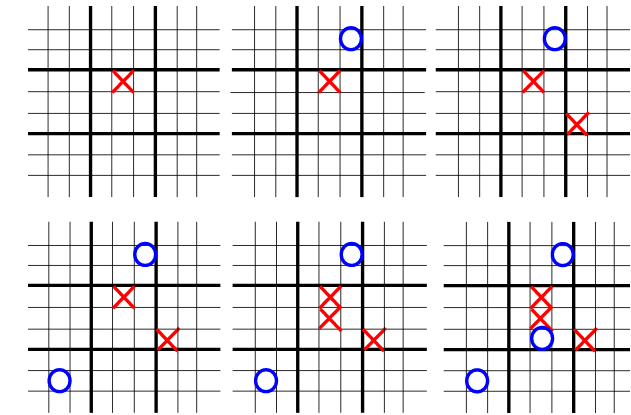
\includegraphics[scale=0.5]{gato.png}
\end{frame}
\begin{frame}{Juego Ganador}
\centering
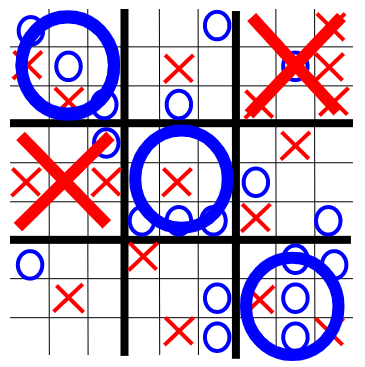
\includegraphics[scale=0.5]{image.png}
\end{frame}

\subsection{Minimax y alpha-beta}
\begin{frame}{Minimax y alpha-beta}
	\textbf{Algoritmo minimax} En teoría de juegos Minimax es un método de decisión para minimizar la pérdida máxima esperada en juegos con adversario y con información perfecta. El funcionamiento de Minimax puede resumirse a como elegir el mejor movimiento para ti mismo; suponiendo que tu contrincante tirará de manera óptima, es decir nos enfrentamos contra un oponente perfecto. \\
	\textbf{Poda alfa-beta} Es una técnica de búsqueda que reduce el número de nodos evaluados en un árbol de juego por el algoritmo Minimax. Partiendo de este hecho, la técnica de poda alfabeta trata de eliminar partes grandes del árbol, aplicándolo a un árbol Minimax estándar, de forma que se devuelva el mismo movimiento que devolvería este, gracias a que la poda de dichas ramas no influye en la decisión final.
\end{frame}
\subsection{Función de Evaluación}
Una parte fundamental del algoritmo alpha-beta es la función de evaluación, la cual debe involucrar toda la información actual de un estado en el juego. Por lo que para el juego Gato×Gato necesitamos de la siguiente información:
\begin{enumerate}
\item Posición del jugador máx
\item Tableros locales ganados por los jugadores máx y mín
\item Tener en cuenta las combinaciones para ganar (por ejemplo las filas, columnas,
y las 2 diagonales) tanto para ganar un tablero local, como para el tablero global
\end{enumerate}
Por lo que podemos dar un ranking de qué cuántos puntos dar por jugada:
\begin{enumerate}
\item score alto por un tablero local ganado.
\item score medio si es posible que en la siguiente jugada se gana un tablero local.
\item score bajo por cada marca en cada tablero local, sin dar situaciones previas.
\end{enumerate}

\section{Resultados}
\begin{frame}
El algoritmo alpha-beta se desempeña de buena manera para este juego el cual puede llegar a generar un árbol lo suficientemente grande si se hiciera búsqueda exhaustiva por lo que dicha mejora fue lo más óptimo sin embargo su desempeño no es el mejor en ciertas situaciones.
\begin{table}
\begin{center}
\begin{tabular}{| c | c |}
Movimineto & Tiempo (s) \\ \hline
Tablero Local Lleno/Ganado & ~14  \\
Ganar tablero Local & ~5\\
Sencillo &  2 \\ \hline
\end{tabular}
\caption{Tiempo aproximado en que la computadora tarda en decidir movimientos específicos}
\label{tab:1}
\end{center}
\end{table}
\textit{El cuadro \ref{tab:1} se obtuvo tras ejecutar el juego con una persona aproximadamente 50 veces.}
\end{frame}

%%%%%%%%%%%%%%%%%%%%%%%%%%%%%%%%%%%%%%%%%%%%%%%
%
%   CLOSING
%
%%%%%%%%%%%%%%%%%%%%%%%%%%%%%%%%%%%%%%%%%%%%%%%
\section{Conclusiones}
\begin{frame}{Conclusiones}
  \centering
Como vemos en juego implementado Gato×Gato debido la cantidad grande de casillas en el tablero global, al momento de hacer búsqueda puede generar una gran cantidad estados posibles en cada momento de selección y a pesar de que en el presente trabajo se usó una mejora de minimax, para tener una mejor eficiencia, aún así no es lo mejor para este juego, como trabajo futuro se propone encontrar una mejor heurística en la función de evaluación para una mejor elección además de implementar el juego probando otras alternativas del estado del arte.

\end{frame}

\begin{frame}[allowframebreaks]{References}
\bibliographystyle{apalike}
\bibliography{bibliography.bib}
\end{frame}

%%
\end{document}
